\section{The Robotic Equipment}\label{sec:robotic-equipment}

\subsection{Safety}
A robot must not have in its construction anything that is dangerous to itself, another robot, or humans.

\subsection{Shape}
A robot must fit inside a 180\,mm diameter cylinder and have a height of 150\,mm or less.
Additionally, a robot's top area must adhere to the Standard Pattern size and surface constraints as described further below in this Law.

\begin{figure}[ht] % ht = here / t = top / b = bottom
	\centering
	\includegraphics[width=0.5\columnwidth]{img/robot_size.png}
	\caption{The maximum robot dimensions}
	\label{fig:robotdimension}
\end{figure}

\subsection{Locomotion}
Robot wheels (or other surfaces that contact the playing surface) must be made of a material that does not harm the playing surface.

\subsection{Wireless Communication}
Robots can use wireless communication to computers or networks located off the field.

\subsection{Team Color}
Before a game, each of the two teams has a color assigned, namely yellow or blue.
All teams must be able to be either yellow or blue color.
The assigned team color is used as the centre marker color for all of the team's robots.
The detailed layout of the markers is described in \autoref{subsec:robotic-equipment-standard-pattern}.

\subsection{Standard Pattern}\label{subsec:robotic-equipment-standard-pattern}
All participating teams must adhere to the given operating requirements of the shared vision system (also see \autoref{sec:field-of-play}).
In particular, teams are required to use a certain set of standardized colors and patterns on top of their robots.

To ensure compatibility with the standardized patterns for the shared vision system, all teams must ensure that all robots have a flat surface with sufficient space available on the top side.
The color of the robot top must be black or dark grey and have a matte (non-shiny) finish to reduce glare.
The SSL-Vision standard pattern is guaranteed to fit within a circle of radius 85\,mm that is linearly cut off on the front side of the robot to a distance of 55\,mm from the centre, as shown in \autoref{fig:robothat}.
Teams must ensure that their robot tops fully enclose this area.

\begin{figure}[ht] % ht = here / t = top / b = bottom
	\centering
	\includegraphics[width=0.8\columnwidth]{img/robot_hat.png}
	\caption{The Minimum Robot Top Area}
	\label{fig:robothat}
\end{figure}

The standard pattern to be used by all teams at RoboCup\added{Soccer Small Size League} is shown in \autoref{fig:stdpattern}.
Note that the organisers reserve the right to change this pattern at any time, if required.
Teams must therefore make sure to still adhere to the standard robot top area size as outlined in \autoref{fig:robothat}.

\begin{figure}[ht] % ht = here / t = top / b = bottom
	\centering
	\includegraphics[width=0.8\columnwidth]{img/standard_pattern2010.png}
	\caption{The Standard Pattern}
	\label{fig:stdpattern}
\end{figure}

Each robot must use the standardized pattern with a unique color assignment
selected from a standardized set of possible color combinations.
No two robots are allowed to use the same color assignment.
The centre dot color determines the team and is either blue or yellow.
All markers must be cut from stock specified by the SSL-Vision
documentation. While teams may acquire the standard color paper in advance of
the competition, limited quantities of standardized colored paper or cardstock for
all required colors will be provided at the competition.
The set of legal color assignments is shown in \autoref{fig:stdcolors}.
Note that the organisers reserve the right to change these color assignments at
any time, if required.

\begin{figure}[ht] % ht = here / t = top / b = bottom
	\centering
	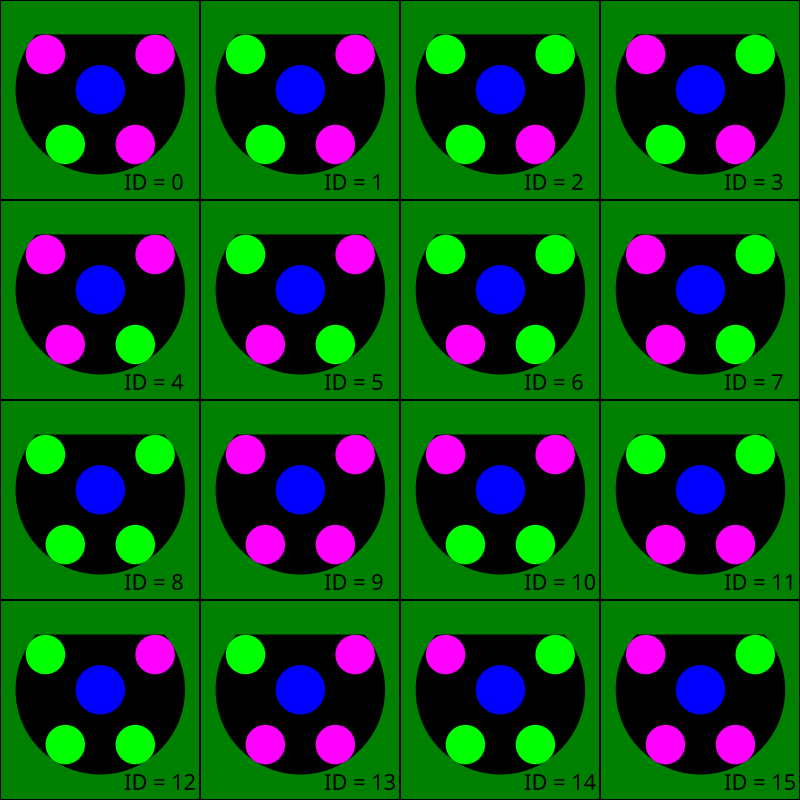
\includegraphics[width=0.8\columnwidth]{img/standard_colors2010.png}
	\caption{The Standard Color Assignments}
	\label{fig:stdcolors}
\end{figure}

Teams are encouraged to select color assignments with IDs 0--7 because they have been experimentally found more stable, as there is no risk that the back two dots ``color-bleed'' into each other.

\subsection{Autonomy}
The robotic equipment is to be fully autonomous.
Human operators are not permitted to enter any information into the equipment during a match, except at half time or during a time-out.

\subsection{Dribbling}
Dribbling devices that actively exert backspin on the ball, which keep the ball in contact with the robot are permitted under certain conditions.
\added{Dribblers that impart a spin to the ball about any axis not parallel to the field plane are not permitted.}
\removed{The spin exerted on the ball must be perpendicular to the plane of the field. Vertical or partially vertical dribbling bars, also known as side dribblers, are not permitted.}
The use of dribbling devices is also restricted as per \autoref{subsec:fouls-and-misconduct-indirect-free-kicks}.

\begin{figure}[ht]
	\centering
	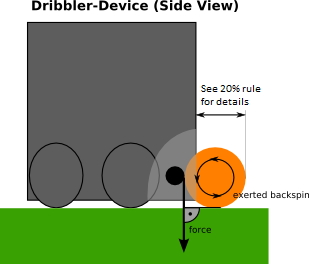
\includegraphics[width=0.5\columnwidth]{img/dribblers_1.png}
	\caption{How a dribbler may work (check \autoref{fig:20-rule} for further detail on the 20\% rule)}
	\label{fig:dribblers}
\end{figure}

\subsection{Infringements/Sanctions}
For any infringement of this Law:

\begin{itemize}
\item play need not be stopped
\item the robot at fault is instructed by the referee to leave the field of play to correct its equipment
\item the robot leaves the field of play when the ball next ceases to be in play
\item any robot required to leave the field of play to correct its equipment does not re-enter without the referee's permission
\item the referee checks that the robot's equipment is correct before allowing it to re-enter the field of play
\item the robot is only allowed to re-enter the field of play when the ball is out of play
\end{itemize}

A robot that has been required to leave the field of play because of an infringement of this Law and that enters (or re-enters) the field of play without the referee's permission \removed{is cautioned and shown the} \added{receives a} yellow card.

\subsection{Restart of Play}
If play is stopped by the referee to administer a caution:

\begin{itemize}
\item the match is restarted by an indirect free kick taken by a robot of the opposing side, from the place where the ball was located when the referee stopped the match
\end{itemize}

\subsection*{Decisions of the Small Size League Technical Committee}
\begin{enumerate}
\item
Participants using wireless communications shall notify the local organising committee of the method of wireless communication, power, and frequency.
The local organising committee shall be notified of any change after registration as soon as possible.

In order to avoid interference, a team should be able to select from two carrier frequencies before the match.
The type of wireless communication shall follow legal regulations of the country where the competition is held.
Compliance with local laws is the responsibility of the competing teams, not the RoboCup Federation.
The type of wireless communication may also be restricted by the local organising committee.
The local organising committee will announce any restrictions to the community as early as possible.

\item
Kicking devices are permitted.

\item
Metal spikes and Velcro are specifically prohibited for the purpose of locomotion.

\item
Bluetooth wireless communication is not allowed.

\item
Adhesives such as glue or tape may not be used for the purpose of ball control or to construct dribblers.
Dribbling devices which use such an adhesive to affix the ball to a robot are considered a violation of \autoref{sec:fouls-and-misconduct}, Decision 4, by ``removing all of the degrees of freedom of the ball''.
In addition, the use of adhesives for any purpose on the robot which results in residue left on the ball or field, is considered as damage and sanctioned as per \autoref{sec:fouls-and-misconduct}.

\item
A rules check will be performed on all robots at the competition prior to the first match.
Any team's robot which is found to violate a rule must be modified to be compliant before it can participate in matches.

\end{enumerate}
